\documentclass[12pt]{exam}

\usepackage{graphicx} % allows for graphics
\usepackage{ifthen}  % for if statements 

\newcommand{\sol}{0} %solution =1 or 0

% LOAD PACKAGES
\usepackage{amsmath} % allows for align env and other things
\usepackage{amssymb} % 
\usepackage{mathtools} % allows for single apostrophe
\usepackage{enumitem} % allows for alpha lettering in enumerated lists
\usepackage{lastpage}
\usepackage{array} % for table alignments
\usepackage{graphicx} % if images are needed

\addpoints

\usepackage{pgfplots} % for surfaces (chapter 7)
\usepackage{tikz-3dplot} 
\pgfplotsset{compat=1.9}
\usetikzlibrary{decorations.pathmorphing,patterns} % for some tikz diagrams
% ~~~~~~~~~~~~~~~~~~~~~~~~~~~~~~~~~~~~
% INITIALS
\newcommand{\Initials}{\textit{\Course, \TestName. Your initials: \underline{\hspace{3cm}}} \vspace{1pt}}

\newcommand{\InitialsLeft}{\noindent \hspace{-18pt}\textit{\Course, \TestName. Your initials: \underline{\hspace{3cm}}} \vspace{1pt}}

\newcommand{\InitialsRight}{\begin{flushright}\textit{\Course, \TestName. Your initials: \underline{\hspace{3cm}}} \vspace{1pt}\end{flushright}}

% ~~~~~~~~~~~~~~~~~~~~~~~~~~~~~~~~~~~~
% INSTRUCTIONS FOR DISTANCE LEARNING WITH NO PROCTOR
\newcommand{\InstructionsFormatAndTiming}{

    \begin{itemize} \setlength\itemsep{.1em}
    
        % \item You should only need 75 min to take the exam, but students will have \Duration to submit the exam, from the time that it is released.
        
        \item {\bf Show your work} and justify your answers for all questions unless stated otherwise.
        
        \item Please write neatly, and use dark and clear writing so that the scan is easy to read. 
        
        \item Please solve the questions in the exam in the order they are given. 
        
        \item You do not need to print the exam. As long as you solve problems in the order they are given you can write your answers on your own paper or by using a tablet. But students can print the exam and write their answers on the printed copy if they prefer. 

        \item Do not type your answers to any part of the exam. 
        
    \end{itemize}

}

\newcommand{\InstructionsSubmission}{

    \begin{itemize} \setlength\itemsep{.1em}
        \item Students should scan their work and submit it through Gradescope. There should be an \textbf{assignment} in Gradescope for this exam. 
        
        \item Work must be submitted by \DueDate. 
        
        \item Please upload your work as a single file. 
        
        \item During the upload process in Gradescope, please indicate which page of your work corresponds to each question. A small number of points will be allocated for this.
    \end{itemize}
}

\newcommand{\InstructionsQuestions}{

    \begin{itemize} \setlength\itemsep{.1em}
        
        \item If there are questions during the exam, students can email their instructor or message them through Canvas. 
        
        \item Our course Piazza forum will be temporarily inactive during the exam. 
        
        \item If you run into any technical issues or any unanticipated emergencies, please email your instructor as soon as you can. 
    
        
    \end{itemize}

}


\newcommand{\InstructionsHonor}{

    \begin{itemize} \setlength\itemsep{.1em}    
        \item Students can use any resources while taking these tests including online calculators and Mathematica
        \item Students cannot communicate with anyone during these tests.
        \item Students cannot use solutions provided from another student or third party. 
        \item In other words: do your own work but you can use technology to solve problems. 
 
    \end{itemize}

}






\newcommand{\GTHonorCode}{Having read the Georgia Institute of Technology Academic Honor Code, I understand and accept my responsibility as a member of the Georgia Tech community to uphold the Honor Code at all times. }



% FANCY HEADERS - MAKE EMPTY
\pagestyle{headandfoot}
\runningfooter{}{}{}


% ADJUST MARGINS FOR DISTANCE LEARNING REQUIREMENTS
\usepackage[tmargin=1.0in,bmargin=1.0in,left=1in,right=1in]{geometry}


% TIKZ DIAGRAMS
\usepackage{color}
\usepackage{tikz}  \usetikzlibrary{arrows} 
\usetikzlibrary{calc} 


% ADJUST FIRST LINE IN PARAGRAPH INDENTATION 
\setlength\parindent{0pt}


% COURSE SPECIFIC INFORMATION
\newcommand{\Course}{Math 2552}
\newcommand{\Instructors}{}

% WHO TO CONTACT DURING EXAM IF QUESTIONS
\newcommand{\InstructorContact}{}

\usepackage{spalign} % Joe Rabinoff's matrix package

\newcommand{\LastPage}{\begin{center}\textit{This page may be used for scratch work. Please indicate clearly if you would like your work on this page to be graded. }\end{center}   }


% DERIVATIVES
\newcommand{\dydt}{{\frac{dy}{dt}}} % 
\newcommand{\dydx}{{\frac{dy}{dx}}} % 
\newcommand{\dydtt}{{\frac{d ^2y}{dt^2}}} % 
\newcommand{\dydxx}{{\frac{d^2y}{dx^2}}} % 
\newcommand{\dydttt}{{\frac{d^3y}{dt^3}}} % 

\newcommand{\ddt}{{\frac{d}{dt}}} % 
\newcommand{\ddx}{{\frac{d}{dx}}} % 
\newcommand{\dudt}{{\frac{du}{dt}}} % 
\newcommand{\dvdx}{{\frac{dv}{dx}}} % 
\newcommand{\dxdt}{{\frac{dx}{dt}}} % 
\newcommand{\dxdtt}{{\frac{d^2x}{dt^2}}} % 
\newcommand{\dzdt}{{\frac{dz}{dt}}} % 



% COLORS FOR DIAGRAMS
\definecolor{DarkBlue}{rgb}{0.0,0.0,0.6} % 
% \definecolor{DarkGreen}{rgb}{0.0,0.3,0.0} % 
% \definecolor{DarkRed}{rgb}{0.6,0.0,0.0} % 

% TEST SPECIFIC INFORMATION
\newcommand{\TestName}{Midterm 2M}
\newcommand{\TestTime}{}
\newcommand{\Duration}{3 hours }
\newcommand{\Points}{}
\newcommand{\DueDate}{12:30 PM ET}


% \usepackage{tikz}
% \usetikzlibrary{shapes,snakes}   
% \usetikzlibrary{arrows,automata}

\begin{document}
    

\vspace*{-1cm}

\begin{center}
{\Large \TestName, \Course }
\end{center}

% \begin{center}    
% {\small
% Instructor: \Instructors \\ Administered on \TestDate. Students should have 3 hours to take this exam. 
% }
% \end{center}


% INSTRUCTIONS FOR STUDENTS
\vspace{2pt}
\begin{center}\textbf{{\large Instructions (PLEASE READ)}}\end{center}
\textbf{Formatting and Timing}
{\small \InstructionsFormatAndTiming}
\textbf{Submission}
{\small \InstructionsSubmission}
\textbf{Questions}
{\small \InstructionsQuestions}
\textbf{Integrity}
{\small \InstructionsHonor}

 % cover page for unproctored exam

\newpage


\InitialsRight

\begin{questions}

    \question[8] 
    Use the method of reduction of order to find a second solution $y_2$ of the given differential equation such that $\{ y_1 , y_2 \}$ is a fundamental set of solutions on the given interval.
    
    $$t^2y'' - 3ty' + 3y = 0, \quad t > 0, \quad y_1(t) = t$$
    
    \newpage    \InitialsLeft
    
        \question[9] Consider a lattice with $3$ lattice points, as in the figure below. 
    
        \begin{center}
            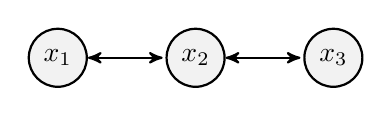
\begin{tikzpicture}
                \begin{scope}[<->,>=stealth',shorten >=1pt,auto,node distance=1.75cm,thick, main node/.style={circle,fill=gray!10,draw}]
                \node[main node] (1) {$x_1$};
                \node[main node] (2) [right of=1] {$x_2$};
                \node[main node] (3) [right of=2] {$x_3$};
                \path[every node/.style={font=\sffamily\small}]
                (1) edge node[below] {} (2)
                (2) edge node [above] {} (3);
                \end{scope}
            \end{tikzpicture}  
        \end{center}  
        
        Let $x_j(t)$ be the number of particles residing at the $j$th lattice point at time $t \ge 0$. Assume that $x_j$ satisfies the following rate equations.
        \begin{align*} 
            \frac{dx_1(t)}{dt} = x_2 - x_1 , \qquad 
            \frac{dx_2(t)}{dt} = x_3 - 2 x_2 + x_1 , \qquad \frac{dx_3(t)}{dt} = x_3
        \end{align*} 
        % Answer the following questions.
        \begin{enumerate} 
            \item[a)] Express the system of equations in the form $\vec x \, ' = A \vec x$. 
                \vspace{2cm}

                \item[b)] Determine the eigenvectors of $A$ and write down the general solution to $\vec x \, ' = A\vec x$. You may use that the eigenvalues of $A$ are $0, 1$ and $-3$. 
                \vspace{10cm} 
                \item[c)] What does the solution converge to as $t \to \infty$? 
        \end{enumerate}
        
        
        
    \newpage \InitialsLeft
        
    \question[10] The position of an undamped spring-mass system satisfies the IVP $$y'' + 5y = 0, \quad y(0) = -1, \quad y'(0) = 0$$ \begin{parts} \part Solve the IVP. \vspace{5cm} \part Sketch the component plot for $y(t)$. \vspace{3cm} \part Sketch the phase portrait for this system. Include the trajectory, $\vec r(t)$, that corresponds to the initial conditions. Clearly label this trajectory and do not forget to label your axes.  \end{parts} 
    
    \newpage \InitialsRight
    
    \question[2] Determine all values of $\alpha$, if any, for which all solutions tend to zero as $t\to\infty$. $$y'' - (2\alpha - 1) y' + (\alpha^2-\alpha+1) y = 0, \quad \alpha \in \mathbb R$$ \vspace{5cm}  % 4.3.47
    
    
    \question[2] % 6.3.4
    State the largest possible interval on which solutions to the IVP are certain to exist. $$(t-2)y'''+ty''+5t^2y'+2t^3y = \ln t, \quad y(1) = 1$$.
    \vspace{3cm}
    

    \newpage \InitialsLeft
    \question[7]  Determine a suitable form for the particular solution, $Y(t)$, to the differential equations if the method of undetermined coefficients is to be used. Do not determine the values of the coefficients or solve the differential equations. 
    \begin{parts}
        \part $y'' - 2y' - 3y = (t^2 + 1)e^{-t}$ \vspace{8cm}
        \part $y'' +2y' - 3y = 3te^t\sin t$
    \end{parts}
    


    \newpage \InitialsRight
    \question[10] Use the variation of parameters method to identify the general solution to \[\vec{x} \, ' = \left( \begin{array}{rr} 2 & 3 \\ 3 & 2 \end{array} \right) \vec{x}  + \left( \begin{array}{r}  0\\ 1\end{array} \right)  \]

    
    \newpage 

    \question[2] A small number of points will be allocated for presentation, neatness, and organization. Please ensure that
    \begin{enumerate}
        % \item your scan is under 5 MB in file size
        \item your work is legible in the scan
        \item your name or initials are at the top of every page
        \item questions are answered in the order in which they were given
        \item during the upload process you have indicated which pages correspond to which question, and made sure that none of your pages are upside down or sideways (you can also change the orientation of the pages when you upload in Gradescope)
    \end{enumerate}
    Ensuring that these criteria are met helps ensure that your exam is graded efficiently and accurately. 
    


    
\end{questions}
    
    Please sign and date the following GT Honor Code statement. \\ 
    \vspace{2pt}
    
    \textbf{Georgia Tech Honor Code}:\ \GTHonorCode
    
    \begin{center}
    \begin{center}
        \def\arraystretch{0.35}%  1 is the default, change whatever you need
        \begin{tabular}{ b{8cm} b{8cm} }
        \vspace{.5cm} \underline{\hspace{7cm}} & \vspace{.5cm} \underline{\hspace{4.5cm}}  \tabularnewline
        \vspace{6pt} signature & \vspace{6pt} date    
        \end{tabular}
    \end{center}
    \end{center}    
\end{document}
